\RequirePackage{fix-cm}
\documentclass[11pt]{article}
\usepackage[fontsize=12pt]{scrextend}
\usepackage{geometry} 
\usepackage{graphicx}
\usepackage{url}
\usepackage{mathtools}
\usepackage{amsmath}
\usepackage{amsfonts}
\usepackage{bigints}
\usepackage{soul,color}
\usepackage{epigraph}
\usepackage[super,numbers,sort&compress]{natbib}
\usepackage[font=scriptsize,labelfont=bf]{caption}
\usepackage[parfill]{parskip}
\usepackage{wrapfig}
%\usepackage{pgfgantt}
\usepackage[hidelinks]{hyperref}
\parskip=8pt
\pagenumbering{gobble}

\bibliographystyle{plos2015}

\geometry{
a4paper,
top=1in,
left=1in,
right=1in,
bottom=1in
} 

\setlength{\parindent}{1.5em}
\setlength{\parskip}{0.1em}

\newcommand{\gb}[1]{{\color{blue}{#1}}}

%	 NOTES ON PROPOSAL
%            1-2pg pre-proposal that includes:
%		general budget
%		relevant personnel (Peter, Gideon, a pdoc tbd)
%		approach
%		deliverables (density, movement, xvalidation w/ previous years/findings)
%			timeline
%		dataset will consist of ~150-200 SNPs


\begin{document}
%
\begin{center}
\textbf{Developing a close-kin mark-recapture model to map black bear population numbers in Michigan (Upper Peninsula)}
\end{center}
%            
\vspace{0.5em}

\noindent Dr. Gideon Bradburd, Dept. of Integrative Biology, Michigan State University\\
\noindent Dr. Peter Ralph, Dept. of Mathematics, University of Oregon

\vspace{1em}

\noindent Getting accurate population size estimates 
for managed or threatened species  
is vital for implementing informed management strategies.
In Michigan, black bears (\textit{Ursus americanus}) 
are managed by harvesting, 
and the hunting license quota is determined by 
estimates of their population size.
Accurate, up-to-date estimates of 
the bear population size in the state 
are therefore a necessary component 
of any effective management plan.

Recent bear population monitoring efforts 
in the state of Michigan have relied on 
capture-mark-recapture (CMR) methods, 
by which a sample of a population is initially marked, 
and an estimate of total population abundance 
can be made from the number of marked individuals 
that are subsequently recaptured (or harvested). 

However, traditional CMR methods are not ideal:  
they require extra fieldwork to do initial population marking; 
the tetracycline biomarker used in marking is no longer permitted; 
and there is a substantial wait time (1-3 years) after the 
initial marking period until population estimates can be made.
Statistical catch-at-age analyses (SCAA), 
a recent advance in CMR methods, 
addresses some of these weaknesses, 
but crucially still requires a costly and time-intensive 
marking field effort.

Using genetic data from sampled individuals 
offers an accurate and cost-effective alternative to CMR 
for estimating population sizes. 
Genetic mark-capture methods can effectively use 
an individual's genetic data in lieu of 
the initial marking effort in a standard CMR; 
researchers may therefore 
only have to do a single round of sampling 
(rather than two), 
or to rely solely on data collected from harvested animals.

\begin{wrapfigure}{r}{.4\textwidth}
    \centering
      \vskip -1em
        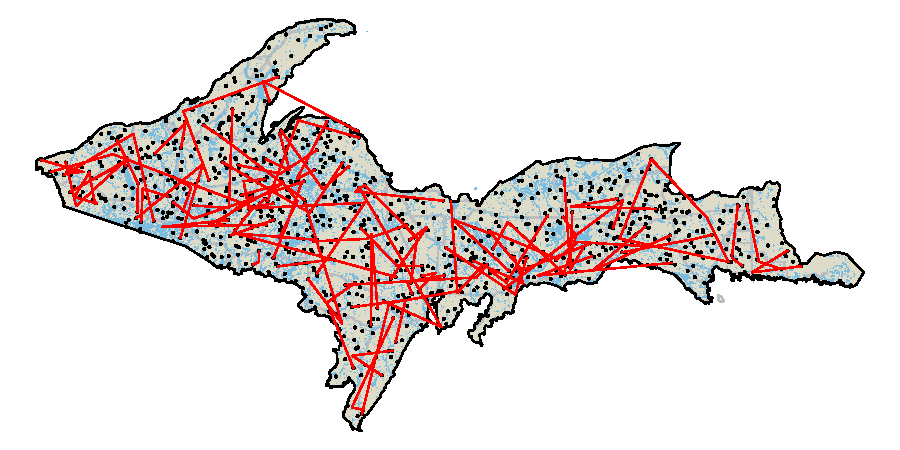
\includegraphics[width=.4\textwidth]{{../sims/bears_K1.0.bear_sibs}.pdf}
        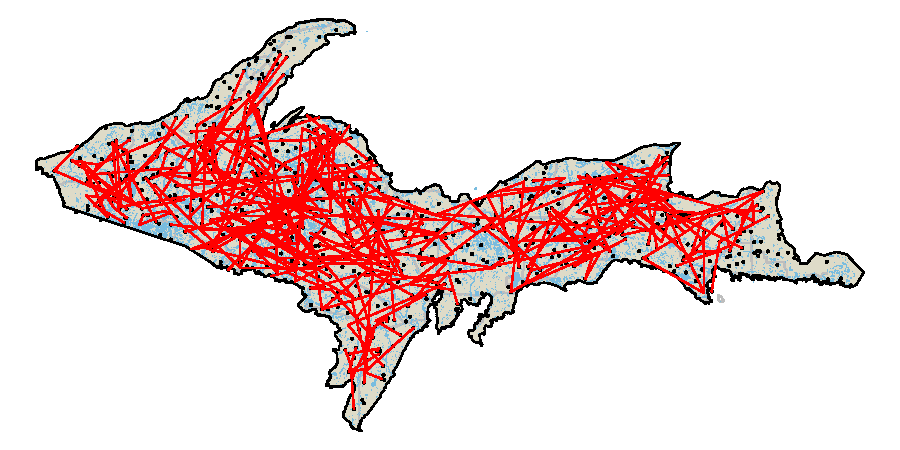
\includegraphics[width=.4\textwidth]{{../sims/bears_K0.25.bear_sibs}.pdf}
    \caption{  \label{fig:maps}
    % NOTE: wrapfigs can't be inside of list environments, which is why this goes to the end
    Locations of sampled bears (black points)
    and relationships of sampled half-sibs (red lines),
    in spatially explicit simulations of sexual, age-structured populations
    with local density-dependent population regulation,
    at two values of local population density.
    In the top figure, a total population of around 14,000 bears resulted in
    73 half-sib pairs out of 1,000 harvested bears,
    while in the lower figure, a total population of around 3,300 resulted in
    216 half-sib pairs out of the same number.
    }
\end{wrapfigure}

Close-kin mark-recapture (CKMR) models 
are an exciting class of genetic mark-recapture methods 
that leverage advances in molecular genetics 
to estimate population size 
from kinship patterns inferred in a genotyped sample.
To build an intuition for how relatedness 
between sampled individuals can be informative 
about total population size, 
we can consider the number of siblings in a sample.
As depicted in Figure~\ref{fig:maps},
a random sample from a population 
with a small number of breeding adults 
is more likely to contain siblings than that 
from a population with a large number of breeding adults; 
the number of sibling-pairs in a sample can 
therefore shed light on adult population sizes 
in the previous generation.

CKMR approaches offer a number of advantages 
over competing models. 
Like all genetic mark recapture models, 
a CKMR approach requires only a single round of sampling, 
which can be achieved through a harvest.
(It would be more accurate to refer to CKMR as 
a Close-Kin Capture method, 
as there is no marking phase, 
so it therefore requires no recapture.)
These methods also avoid some types of bias 
that can be introduced into CMR methods due to 
heterogeneity in capture/recapture probability.
Moreover, by focusing on multiple pedigree connections 
(e.g., half-sib relationships, 
in addition to parent-offspring and full-sib) 
they allow a researcher to study unsampled individuals.

Here, we propose to develop a CKMR model 
for black bears in Michigan's Upper Peninsula (UP) 
for use by the Michigan Department of Natural Resources.
This model, which will account for 
variable fecundity and capture probability, 
as well as non-sparse sampling, 
will generate population size estimates 
for the adult, pre-harvest black bear population in the UP. 
Because spatial structure in the bear population might impact 
population size estimates, 
we will also extend existing CKMR models 
to incorporate geography.
In addition to generating estimates of total population size 
that are robust to the spatial structure of the pedigree, 
this spatial model will also generate maps of estimated 
population density, 
and has the potential to shed light 
on other demographic parameters as well.
This model will be extensively tested using spatially explicit,  
forward-time simulations carried out on a map of the UP. 
To demonstrate the feasibility of this approach, 
we have included sample simulations 
of the bear population in the UP (Fig \ref{fig:maps}).
Simulations were run with SLiM \citep{haller2018forward},
and have many realistic features 
(e.g., nonuniform density and local post-natal dispersal) 
but are only proof-of-concept.
Code available at \url{https://github.com/petrelharp/howmanybears}.
Biological parameters used to simulate these test data 
will be informed by previous demographic and ecological 
research on Michigan black bears \citep{moore2014application}.
These simulations will be used both to 
validate the proposed inference procedure 
and to explore the sensitivity of the output to model assumptions 
(all model assumptions will be listed in the model documentation).

To disseminate the results of this new model, 
we will implement it in well-documented scripts 
that produce templated reports and graphical output
for easy use by the DNR, 
and provide accompanying vignettes 
and a video walk-through demonstration. 
We will also engage in educational trainings with state biologists, 
and assist in outreach with 
administrators, commissioners, and stakeholders.

We are confident that we will be able to 
carry out the proposed work in the timeline below (Fig \ref{timeline}).
Both PIs Bradburd and Ralph have extensive 
experience developing statistical methods \citep{bedassle, SpaceMix, bradburd2018inferring} -- 
with a particular focus on spatial population genetics \citep{bradburd2019spatial, Battey_etal_2020} -- 
and implementing them as documented software packages.
In addition, the PIs have collaborated previously 
on black bear research \citep{bradburd2018inferring}
and on developing management plans 
for government agencies \citep{shaffer2017desert}, 
and have recently co-written a review discussing how to link properties of the pedigree
to population demography and dynamics \citep{bradburd2019spatial}.
% value added: all inds simultaneously vs. one dyad at a time? ; MI-specifc simulation framework

\begin{figure}[h!]
    \centering
         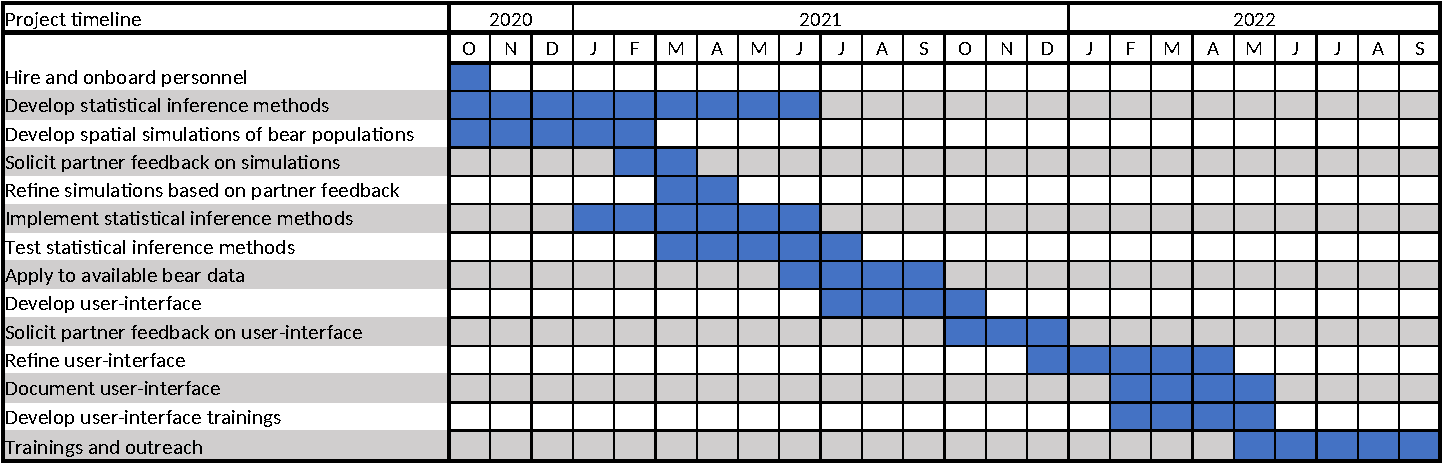
\includegraphics[width=0.9\linewidth]{bear_gantt_chart.pdf}
        \caption{
		Timeline of proposed work.
        }
        \label{timeline}
\end{figure}

\clearpage
\bibliography{references.bib}
\end{document}